%%%% Paramétrage du TD %%%%
\def\xxactivite{Révisions \ifprof -- Corrigé \else \fi} % \normalsize \vspace{-.4cm}
\def\xxauteur{\textsl{Xavier Pessoles}}


\def\xxnumchapitre{Révision cinématique \vspace{.2cm}}
\def\xxchapitre{\hspace{.12cm} Résolution cinématique}
\def\xxonglet{\textsf{Rév -- Stat}}
\def\xxactivite{Application 01}
\def\xxauteur{\textsl{Xavier Pessoles}}

\def\xxpied{%
Révision cinématique \\
Fiche  2 -- \xxactivite%
}

\def\xxtitreexo{Capsuleuse de bocaux  \ifnormal $\star$ \else \fi \ifdifficile $\star\star$ \else \fi \iftdifficile $\star\star\star$ \else \fi}

\def\xxsourceexo{\hspace{.2cm} \footnotesize{Xavier Pessoles}}


\def\xxcompetences{%
\textsl{%
\textbf{Savoirs et compétences :}\\} \vspace{-.5cm}
%\begin{itemize}
%\item \textit{Res2.C18} : principe fondamental de la statique;
%\item \textit{Res2.C19} : équilibre d’un solide, d’un ensemble de solides;
%\item \textit{Res2.C20} : théorème des actions réciproques.
%\end{itemize}
}


\def\xxfigures{
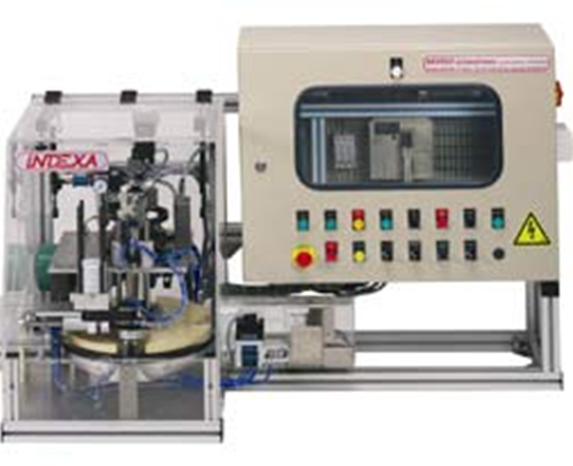
\includegraphics[width=.6\textwidth]{capsuleuse}
}%figues de la page de garde




\iflivret
\pagestyle{empty}


%%%%%%%% PAGE DE GARDE COURS
\ifcours
% ==== BANDEAU DES TITRES ==== 
\begin{tikzpicture}[remember picture,overlay]
\node at (current page.north west)
{\begin{tikzpicture}[remember picture,overlay]
\node[anchor=north west,inner sep=0pt] at (0,0) {\includegraphics[width=\paperwidth]{\thechapterimage}};
\draw[anchor=west] (-2cm,-8cm) node [line width=2pt,rounded corners=15pt,draw=ocre,fill=white,fill opacity=0.6,inner sep=40pt]{\strut\makebox[22cm]{}};
\draw[anchor=west] (1cm,-8cm) node {\huge\sffamily\bfseries\color{black} %
\begin{minipage}{1cm}
\rotatebox{90}{\LARGE\sffamily\textsc{\color{ocre}\textbf{\xxnumpartie}}}
\end{minipage} \hfill
\begin{minipage}[c]{14cm}
\begin{titrepartie}
\begin{flushright}
\renewcommand{\baselinestretch}{1.1} 
\Large\sffamily\textsc{\textbf{\xxpartie}}
\renewcommand{\baselinestretch}{1} 
\end{flushright}
\end{titrepartie}
\end{minipage} \hfill
\begin{minipage}[c]{3.5cm}
{\large\sffamily\textsc{\textbf{\color{ocre} \discipline}}}
\end{minipage} 
 };
\end{tikzpicture}};
\end{tikzpicture}
% ==== FIN BANDEAU DES TITRES ==== 


% ==== ONGLET 
\begin{tikzpicture}[overlay]
\node[shape=rectangle, 
      rounded corners = .25 cm,
	  draw= ocre,
	  line width=2pt, 
	  fill = ocre!10,
	  minimum width  = 2.5cm,
	  minimum height = 3cm,] at (18.3cm,0) {};
\node at (17.7cm,0) {\rotatebox{90}{\textbf{\Large\color{ocre}{\classe}}}};
%{};
\end{tikzpicture}
% ==== FIN ONGLET 


\vspace{3.5cm}

\begin{tikzpicture}[remember picture,overlay]
\draw[anchor=west] (-2cm,-6cm) node {\huge\sffamily\bfseries\color{black} %
\begin{minipage}{2cm}
\begin{center}
\LARGE\sffamily\textsc{\color{ocre}\textbf{\xxactivite}}
\end{center}
\end{minipage} \hfill
\begin{minipage}[c]{15cm}
\begin{titrechapitre}
\renewcommand{\baselinestretch}{1.1} 
\Large\sffamily\textsc{\textbf{\xxnumchapitre}}

\Large\sffamily\textsc{\textbf{\xxchapitre}}
\vspace{.5cm}

\renewcommand{\baselinestretch}{1} 
\normalsize\normalfont
\xxcompetences
\end{titrechapitre}
\end{minipage}  };
\end{tikzpicture}
\vfill

\begin{flushright}
\begin{minipage}[c]{.3\linewidth}
\begin{center}
\xxfigures
\end{center}
\end{minipage}\hfill
\begin{minipage}[c]{.6\linewidth}
\startcontents
%\printcontents{}{1}{}
\printcontents{}{1}{}
\end{minipage}
\end{flushright}

\begin{tikzpicture}[remember picture,overlay]
\draw[anchor=west] (4.5cm,-.7cm) node {
\begin{minipage}[c]{.2\linewidth}
\begin{flushright}

\includegraphics[width=2cm]{logoCC}
\end{flushright}
\end{minipage}
\begin{minipage}[c]{.2\linewidth}
\textsl{\xxauteur} \\
\textsl{\classe}
\end{minipage}
 };
\end{tikzpicture}

\newpage
\pagestyle{fancy}

%\newpage
%\pagestyle{fancy}

\else
\fi
%% FIN PAGE DE GARDE DES COURS

%%%%%%%% PAGE DE GARDE TD
\iftd
%\begin{tikzpicture}[remember picture,overlay]
%\node at (current page.north west)
%{\begin{tikzpicture}[remember picture,overlay]
%\draw[anchor=west] (-2cm,-3.25cm) node [line width=2pt,rounded corners=15pt,draw=ocre,fill=white,fill opacity=0.6,inner sep=40pt]{\strut\makebox[22cm]{}};
%\draw[anchor=west] (1cm,-3.25cm) node {\huge\sffamily\bfseries\color{black} %
%\begin{minipage}{1cm}
%\rotatebox{90}{\LARGE\sffamily\textsc{\color{ocre}\textbf{\xxnumpartie}}}
%\end{minipage} \hfill
%\begin{minipage}[c]{13.5cm}
%\begin{titrepartie}
%\begin{flushright}
%\renewcommand{\baselinestretch}{1.1} 
%\Large\sffamily\textsc{\textbf{\xxpartie}}
%\renewcommand{\baselinestretch}{1} 
%\end{flushright}
%\end{titrepartie}
%\end{minipage} \hfill
%\begin{minipage}[c]{3.5cm}
%{\large\sffamily\textsc{\textbf{\color{ocre} \discipline}}}
%\end{minipage} 
% };
%\end{tikzpicture}};
%\end{tikzpicture}

%%%%%%%%%% PAGE DE GARDE TD %%%%%%%%%%%%%%%
%\begin{tikzpicture}[overlay]
%\node[shape=rectangle, 
%      rounded corners = .25 cm,
%	  draw= ocre,
%	  line width=2pt, 
%	  fill = ocre!10,
%	  minimum width  = 2.5cm,
%	  minimum height = 2.5cm,] at (18.5cm,0) {};
%\node at (17.7cm,0) {\rotatebox{90}{\textbf{\Large\color{ocre}{\classe}}}};
%%{};
%\end{tikzpicture}

% PARTIE ET CHAPITRE
%\begin{tikzpicture}[remember picture,overlay]
%\draw[anchor=west] (-1cm,-2.1cm) node {\large\sffamily\bfseries\color{black} %
%\begin{minipage}[c]{15cm}
%\begin{flushleft}
%\xxnumchapitre \\
%\xxchapitre
%\end{flushleft}
%\end{minipage}  };
%\end{tikzpicture}

% BANDEAU EXO
\iflivret % SI LIVRET
\begin{tikzpicture}[remember picture,overlay]
\draw[anchor=west] (-2cm,-3.3cm) node {\huge\sffamily\bfseries\color{black} %
\begin{minipage}{5cm}
\begin{center}
\LARGE\sffamily\color{ocre}\textbf{\textsc{\xxactivite}}

\begin{center}
\xxfigures
\end{center}

\end{center}
\end{minipage} \hfill
\begin{minipage}[c]{12cm}
\begin{titrechapitre}
\renewcommand{\baselinestretch}{1.1} 
\large\sffamily\textbf{\textsc{\xxtitreexo}}

\small\sffamily{\textbf{\textit{\color{black!70}\xxsourceexo}}}
\vspace{.5cm}

\renewcommand{\baselinestretch}{1} 
\normalsize\normalfont
\xxcompetences
\end{titrechapitre}
\end{minipage}};
\end{tikzpicture}
\else % ELSE NOT LIVRET
\begin{tikzpicture}[remember picture,overlay]
\draw[anchor=west] (-2cm,-4.5cm) node {\huge\sffamily\bfseries\color{black} %
\begin{minipage}{5cm}
\begin{center}
\LARGE\sffamily\color{ocre}\textbf{\textsc{\xxactivite}}

\begin{center}
\xxfigures
\end{center}

\end{center}
\end{minipage} \hfill
\begin{minipage}[c]{12cm}
\begin{titrechapitre}
\renewcommand{\baselinestretch}{1.1} 
\large\sffamily\textbf{\textsc{\xxtitreexo}}

\small\sffamily{\textbf{\textit{\color{black!70}\xxsourceexo}}}
\vspace{.5cm}

\renewcommand{\baselinestretch}{1} 
\normalsize\normalfont
\xxcompetences
\end{titrechapitre}
\end{minipage}};
\end{tikzpicture}

\fi

\else   % FIN IF TD
\fi


%%%%%%%% PAGE DE GARDE FICHE
\iffiche
\begin{tikzpicture}[remember picture,overlay]
\node at (current page.north west)
{\begin{tikzpicture}[remember picture,overlay]
\draw[anchor=west] (-2cm,-2.25cm) node [line width=2pt,rounded corners=15pt,draw=ocre,fill=white,fill opacity=0.6,inner sep=40pt]{\strut\makebox[22cm]{}};
\draw[anchor=west] (1cm,-2.25cm) node {\huge\sffamily\bfseries\color{black} %
\begin{minipage}{1cm}
\rotatebox{90}{\LARGE\sffamily\textsc{\color{ocre}\textbf{\xxnumpartie}}}
\end{minipage} \hfill
\begin{minipage}[c]{14cm}
\begin{titrepartie}
\begin{flushright}
\renewcommand{\baselinestretch}{1.1} 
\large\sffamily\textsc{\textbf{\xxpartie} \\} 

\vspace{.2cm}

\normalsize\sffamily\textsc{\textbf{\xxnumchapitre -- \xxchapitre}}
\renewcommand{\baselinestretch}{1} 
\end{flushright}
\end{titrepartie}
\end{minipage} \hfill
\begin{minipage}[c]{3.5cm}
{\large\sffamily\textsc{\textbf{\color{ocre} \discipline}}}
\end{minipage} 
 };
\end{tikzpicture}};
\end{tikzpicture}

\iflivret
\begin{tikzpicture}[overlay]
\node[shape=rectangle, 
      rounded corners = .25 cm,
	  draw= ocre,
	  line width=2pt, 
	  fill = ocre!10,
	  minimum width  = 2.5cm,
	  minimum height = 2.5cm,] at (18.5cm,.5cm) {};
\node at (17.9cm,.5cm) {\rotatebox{90}{\textsf{\textbf{\large\color{ocre}{\classe}}}}};
%{};
\end{tikzpicture}
\else
\begin{tikzpicture}[overlay]
\node[shape=rectangle, 
      rounded corners = .25 cm,
	  draw= ocre,
	  line width=2pt, 
	  fill = ocre!10,
	  minimum width  = 2.5cm,
%	  minimum height = 2.5cm,] at (18.5cm,1.1cm) {};
	  minimum height = 2.5cm,] at (18.6cm,0.5cm) {};
\node at (18cm,0.5cm) {\rotatebox{90}{\textsf{\textbf{\large\color{ocre}{\classe}}}}};
%{};
\end{tikzpicture}

\fi

\else
\fi



\else
\pagestyle{empty}


%%%%%%%% PAGE DE GARDE COURS
\ifcours
% ==== BANDEAU DES TITRES ==== 
\begin{tikzpicture}[remember picture,overlay]
\node at (current page.north west)
{\begin{tikzpicture}[remember picture,overlay]
\node[anchor=north west,inner sep=0pt] at (0,0) {\includegraphics[width=\paperwidth]{\thechapterimage}};
\draw[anchor=west] (-2cm,-8cm) node [line width=2pt,rounded corners=15pt,draw=ocre,fill=white,fill opacity=0.6,inner sep=40pt]{\strut\makebox[22cm]{}};
\draw[anchor=west] (1cm,-8cm) node {\huge\sffamily\bfseries\color{black} %
\begin{minipage}{1cm}
\rotatebox{90}{\LARGE\sffamily\textsc{\color{ocre}\textbf{\xxnumpartie}}}
\end{minipage} \hfill
\begin{minipage}[c]{14cm}
\begin{titrepartie}
\begin{flushright}
\renewcommand{\baselinestretch}{1.1} 
\Large\sffamily\textsc{\textbf{\xxpartie}}
\renewcommand{\baselinestretch}{1} 
\end{flushright}
\end{titrepartie}
\end{minipage} \hfill
\begin{minipage}[c]{3.5cm}
{\large\sffamily\textsc{\textbf{\color{ocre} \discipline}}}
\end{minipage} 
 };
\end{tikzpicture}};
\end{tikzpicture}
% ==== FIN BANDEAU DES TITRES ==== 


% ==== ONGLET 
\begin{tikzpicture}[overlay]
\node[shape=rectangle, 
      rounded corners = .25 cm,
	  draw= ocre,
	  line width=2pt, 
	  fill = ocre!10,
	  minimum width  = 2.5cm,
	  minimum height = 3cm,] at (18.3cm,0) {};
\node at (17.7cm,0) {\rotatebox{90}{\textbf{\Large\color{ocre}{\classe}}}};
%{};
\end{tikzpicture}
% ==== FIN ONGLET 


\vspace{3.5cm}

\begin{tikzpicture}[remember picture,overlay]
\draw[anchor=west] (-2cm,-6cm) node {\huge\sffamily\bfseries\color{black} %
\begin{minipage}{2cm}
\begin{center}
\LARGE\sffamily\textsc{\color{ocre}\textbf{\xxactivite}}
\end{center}
\end{minipage} \hfill
\begin{minipage}[c]{15cm}
\begin{titrechapitre}
\renewcommand{\baselinestretch}{1.1} 
\Large\sffamily\textsc{\textbf{\xxnumchapitre}}

\Large\sffamily\textsc{\textbf{\xxchapitre}}
\vspace{.5cm}

\renewcommand{\baselinestretch}{1} 
\normalsize\normalfont
\xxcompetences
\end{titrechapitre}
\end{minipage}  };
\end{tikzpicture}
\vfill

\begin{flushright}
\begin{minipage}[c]{.3\linewidth}
\begin{center}
\xxfigures
\end{center}
\end{minipage}\hfill
\begin{minipage}[c]{.6\linewidth}
\startcontents
%\printcontents{}{1}{}
\printcontents{}{1}{}
\end{minipage}
\end{flushright}

\begin{tikzpicture}[remember picture,overlay]
\draw[anchor=west] (4.5cm,-.7cm) node {
\begin{minipage}[c]{.2\linewidth}
\begin{flushright}

\includegraphics[width=2cm]{logoCC}
\end{flushright}
\end{minipage}
\begin{minipage}[c]{.2\linewidth}
\textsl{\xxauteur} \\
\textsl{\classe}
\end{minipage}
 };
\end{tikzpicture}

\newpage
\pagestyle{fancy}

%\newpage
%\pagestyle{fancy}

\else
\fi
%% FIN PAGE DE GARDE DES COURS

%%%%%%%% PAGE DE GARDE TD
\iftd
%\begin{tikzpicture}[remember picture,overlay]
%\node at (current page.north west)
%{\begin{tikzpicture}[remember picture,overlay]
%\draw[anchor=west] (-2cm,-3.25cm) node [line width=2pt,rounded corners=15pt,draw=ocre,fill=white,fill opacity=0.6,inner sep=40pt]{\strut\makebox[22cm]{}};
%\draw[anchor=west] (1cm,-3.25cm) node {\huge\sffamily\bfseries\color{black} %
%\begin{minipage}{1cm}
%\rotatebox{90}{\LARGE\sffamily\textsc{\color{ocre}\textbf{\xxnumpartie}}}
%\end{minipage} \hfill
%\begin{minipage}[c]{13.5cm}
%\begin{titrepartie}
%\begin{flushright}
%\renewcommand{\baselinestretch}{1.1} 
%\Large\sffamily\textsc{\textbf{\xxpartie}}
%\renewcommand{\baselinestretch}{1} 
%\end{flushright}
%\end{titrepartie}
%\end{minipage} \hfill
%\begin{minipage}[c]{3.5cm}
%{\large\sffamily\textsc{\textbf{\color{ocre} \discipline}}}
%\end{minipage} 
% };
%\end{tikzpicture}};
%\end{tikzpicture}

%%%%%%%%%% PAGE DE GARDE TD %%%%%%%%%%%%%%%
%\begin{tikzpicture}[overlay]
%\node[shape=rectangle, 
%      rounded corners = .25 cm,
%	  draw= ocre,
%	  line width=2pt, 
%	  fill = ocre!10,
%	  minimum width  = 2.5cm,
%	  minimum height = 2.5cm,] at (18.5cm,0) {};
%\node at (17.7cm,0) {\rotatebox{90}{\textbf{\Large\color{ocre}{\classe}}}};
%%{};
%\end{tikzpicture}

% PARTIE ET CHAPITRE
%\begin{tikzpicture}[remember picture,overlay]
%\draw[anchor=west] (-1cm,-2.1cm) node {\large\sffamily\bfseries\color{black} %
%\begin{minipage}[c]{15cm}
%\begin{flushleft}
%\xxnumchapitre \\
%\xxchapitre
%\end{flushleft}
%\end{minipage}  };
%\end{tikzpicture}

% BANDEAU EXO
\iflivret % SI LIVRET
\begin{tikzpicture}[remember picture,overlay]
\draw[anchor=west] (-2cm,-3.3cm) node {\huge\sffamily\bfseries\color{black} %
\begin{minipage}{5cm}
\begin{center}
\LARGE\sffamily\color{ocre}\textbf{\textsc{\xxactivite}}

\begin{center}
\xxfigures
\end{center}

\end{center}
\end{minipage} \hfill
\begin{minipage}[c]{12cm}
\begin{titrechapitre}
\renewcommand{\baselinestretch}{1.1} 
\large\sffamily\textbf{\textsc{\xxtitreexo}}

\small\sffamily{\textbf{\textit{\color{black!70}\xxsourceexo}}}
\vspace{.5cm}

\renewcommand{\baselinestretch}{1} 
\normalsize\normalfont
\xxcompetences
\end{titrechapitre}
\end{minipage}};
\end{tikzpicture}
\else % ELSE NOT LIVRET
\begin{tikzpicture}[remember picture,overlay]
\draw[anchor=west] (-2cm,-4.5cm) node {\huge\sffamily\bfseries\color{black} %
\begin{minipage}{5cm}
\begin{center}
\LARGE\sffamily\color{ocre}\textbf{\textsc{\xxactivite}}

\begin{center}
\xxfigures
\end{center}

\end{center}
\end{minipage} \hfill
\begin{minipage}[c]{12cm}
\begin{titrechapitre}
\renewcommand{\baselinestretch}{1.1} 
\large\sffamily\textbf{\textsc{\xxtitreexo}}

\small\sffamily{\textbf{\textit{\color{black!70}\xxsourceexo}}}
\vspace{.5cm}

\renewcommand{\baselinestretch}{1} 
\normalsize\normalfont
\xxcompetences
\end{titrechapitre}
\end{minipage}};
\end{tikzpicture}

\fi

\else   % FIN IF TD
\fi


%%%%%%%% PAGE DE GARDE FICHE
\iffiche
\begin{tikzpicture}[remember picture,overlay]
\node at (current page.north west)
{\begin{tikzpicture}[remember picture,overlay]
\draw[anchor=west] (-2cm,-2.25cm) node [line width=2pt,rounded corners=15pt,draw=ocre,fill=white,fill opacity=0.6,inner sep=40pt]{\strut\makebox[22cm]{}};
\draw[anchor=west] (1cm,-2.25cm) node {\huge\sffamily\bfseries\color{black} %
\begin{minipage}{1cm}
\rotatebox{90}{\LARGE\sffamily\textsc{\color{ocre}\textbf{\xxnumpartie}}}
\end{minipage} \hfill
\begin{minipage}[c]{14cm}
\begin{titrepartie}
\begin{flushright}
\renewcommand{\baselinestretch}{1.1} 
\large\sffamily\textsc{\textbf{\xxpartie} \\} 

\vspace{.2cm}

\normalsize\sffamily\textsc{\textbf{\xxnumchapitre -- \xxchapitre}}
\renewcommand{\baselinestretch}{1} 
\end{flushright}
\end{titrepartie}
\end{minipage} \hfill
\begin{minipage}[c]{3.5cm}
{\large\sffamily\textsc{\textbf{\color{ocre} \discipline}}}
\end{minipage} 
 };
\end{tikzpicture}};
\end{tikzpicture}

\iflivret
\begin{tikzpicture}[overlay]
\node[shape=rectangle, 
      rounded corners = .25 cm,
	  draw= ocre,
	  line width=2pt, 
	  fill = ocre!10,
	  minimum width  = 2.5cm,
	  minimum height = 2.5cm,] at (18.5cm,.5cm) {};
\node at (17.9cm,.5cm) {\rotatebox{90}{\textsf{\textbf{\large\color{ocre}{\classe}}}}};
%{};
\end{tikzpicture}
\else
\begin{tikzpicture}[overlay]
\node[shape=rectangle, 
      rounded corners = .25 cm,
	  draw= ocre,
	  line width=2pt, 
	  fill = ocre!10,
	  minimum width  = 2.5cm,
%	  minimum height = 2.5cm,] at (18.5cm,1.1cm) {};
	  minimum height = 2.5cm,] at (18.6cm,0.5cm) {};
\node at (18cm,0.5cm) {\rotatebox{90}{\textsf{\textbf{\large\color{ocre}{\classe}}}}};
%{};
\end{tikzpicture}

\fi

\else
\fi



\fi
\setlength{\columnseprule}{.1pt}

\pagestyle{fancy}
\thispagestyle{plain}

\ifprof
\vspace{5cm}
\else
\vspace{4cm}
\fi

\def\columnseprulecolor{\color{ocre}}
\setlength{\columnseprule}{0.4pt} 

%%%%%%%%%%%%%%%%%%%%%%%

\setcounter{exo}{0}



\ifprof
\else
\begin{multicols}{2}
\fi


Le conditionnement de nombreux produits alimentaires est réalisé dans des bocaux en verre fermés par des capsules vissées. La société RAVOUX, spécialisée dans le conditionnement, a créé ce prototype afin d'optimiser ses machines de production. Elle est donc équipée de nombreux capteurs permettant, via un ordinateur, d'optimiser les paramètres de production tels que qualité totale, production maximale, ...

Le système de laboratoire proposé s'insère dans une chaîne de conditionnement de produits alimentaires, entre l'unité de remplissage des bocaux et le poste d'étiquetage. Sa fonction principale est la «fermeture étanche de bocaux préalablement remplis de produits alimentaires»


%
%Ce système comprend plusieurs parties :
%\begin{itemize}
%\item un convoyeur linéaire d'alimentation des bocaux ;
%\item un système électromécanique de transfert et d'indexation des bocaux (moto-réducteur, mécanisme à Croix de Malte, étoile de transfert) ;
%\item un magasin de stockage des capsules ;
%\item une partie opérative pneumatique de pose et de vissage des capsules - vérin V1, tête de vissage comprenant les vérins V2 et VR, ventouse et vacuostat (le vacuostat est une cellule permettant d'assurer la mise en dépression de la ventouse afin d'effectuer la préhension de la capsule) ;
%\item un vérin de serrage des bocaux sous la tête de vissage ;
%\item un convoyeur linéaire d'évacuation des bocaux ;
%\item une partie commande par automate programmable Télémécanique TSX 37-10 64 entrées/sorties et un pupitre de commande.
%\end{itemize}

\begin{center}
 \includegraphics[width=.8\linewidth]{systeme3}
\end{center}


On s'intéresse ici au système de croix de Malte. Il permet d'obtenir une rotation discontinue à partir d'un mouvement de rotation continue. Ainsi, pendant que la croix de Malte ne tourne pas, le système peut agir sur la matière d'\oe{}uvre (flacon).

Lors de la rotation de la croix de Malte, la capsuleuse déplace deux flacons. Afin d'accroître la productivité, il faut diminuer la durée de cette phase. Cependant, si la croix de Malte tourne trop vite, les flacons basculent ce qui entraîne un mauvais fonctionnement du système. Ainsi, on désire que la \textbf{vitesse de la croix soit inférieure à 50 tours/minute}. 



\subsection*{Modélisation sans galet}

Afin de modéliser le système à croix de malte, on propose le schéma cinématique ci-contre. 


On note :
\begin{itemize}
\item $\mathcal{R}=\left( O,\vect{x_0},\vect{y_0},\vect{z_0}\right)$ le repère lié au bâti $S_0$. On note $\vect{OB}=-L\vect{x_0}$ avec $L = \SI{145}{mm}$;
\item $\mathcal{R}_1=\left( O,\vect{x_1},\vect{y_1},\vect{z_1}\right)$ le repère lié à l'arbre $S_1$. On pose $\vect{OA}=R\vect{y_1}$  avec $R =\SI{141}{mm}$ et $\alpha = \left( \vect{x_0}, \vect{x_1}\right)$. L'arbre $S_1$ est lié au motoréducteur de la capsuleuse. On a : $\dot{\alpha} = \SI{10}{tr/min}$;
\item  $\mathcal{R}_2=\left( B,\vect{x_2},\vect{y_2},\vect{z_2}\right)$ le repère lié à l'arbre $S_2$. On pose $\vect{BA}=\lambda(t)\vect{x_2}$,  $\vect{AI}=r\vect{y_2}$ et $\beta = \left( \vect{x_0}, \vect{x_2}\right)$;
\end{itemize}


\begin{center}
 \includegraphics[width=\linewidth]{schema1}
\end{center}


%\subparagraph{}
%\textit{Indiquer une différence majeure entre le système réel et le système modélisé.}

\subparagraph{}
\textit{Donner le paramétrage associé au schéma cinématique.}

\ifprof%
\begin{corrige}
\begin{center}
 \includegraphics[width=.4\linewidth]{param1}
\end{center}
\end{corrige}
\else \fi

\subparagraph{}
\textit{\'Etablir la loi entrée/sortie du système.}


\ifprof%
\begin{corrige}

On a :
$$ \vect{OA} + \vect{AB} + \vect{BO} = \vect{0} \Longleftrightarrow 
R\vect{y_1} - \lambda(t)\vect{x_2} + L \vect{x_0} = \vect{0}
$$
En projetant sur $\vect{x_0}$ et $\vect{y_0}$ on a :
$$
\left\{
\begin{array}{l}
- R \sin \alpha(t) - \lambda(t) \cos\beta(t) + L = 0\\
R\cos\alpha(t) - \lambda(t)\sin \beta(t)=0
\end{array}
\right.
$$
Suivant le cas, on peut donc avoir $\alpha$ en fonction de $\beta$ ou $\lambda$ en fonction de $\alpha$ ou $\beta$ :
$$
\tan \beta = \dfrac{R\cos\alpha}{L-R\sin\alpha}
$$

$$
\lambda(t)^2 = R^2 + L^2 - 2RL \sin\alpha
$$
\end{corrige}
\else \fi

\subparagraph{}
\textit{Donner une méthode permettant de valider la cahier des charges vis à vis de la vitesse de rotation de la croix de Malte.}


\ifprof%
\begin{corrige}

On peut calculer : 
$$
\dot{\beta} = \dfrac{R^2\dot{\alpha} - LR\dot{\alpha}\sin\alpha }{L^2-2RL\sin\alpha + R^2}
$$

Le tracé Excel permet de valider que la vitesse de rotation de la croix de Malte reste inférieure à 50 tours par minute.

\end{corrige}
\else \fi


\subparagraph{}
%\textit{Donner l'expression du torseur cinématique de $S_1$ par rapport à $S_0$ au point $I$.}
\textit{Donner l'expression de $\vect{V(I,S_1/S_0)}$ et $\vecto{S_1}{S_0}$.}

\ifprof%
\begin{corrige}

$$\{\mathcal{V}(S_1/S_0)\} = 
\left\{
\begin{array}{l}
\vect{\Omega(S_1/S_0)} = \dot{\alpha}\vect{z_0} \\
\vect{V(O,S_1/S_0)} = \vect{0}
\end{array}
\right\}_O =
\left\{
\begin{array}{l}
\vect{\Omega(S_1/S_0)} = \dot{\alpha}\vect{z_0} \\
\vect{V(I,S_1/S_0)} = \vect{IO} \wedge \dot{\alpha}\vect{z_0}
\end{array}
\right\}_I
$$

$$
\vect{V(I,S_1/S_0)} =\left( -R\vect{y_1} - r \vect{y_2} \right) \wedge \dot{\alpha}\vect{z_0} =- R\dot{\alpha}\vect{x_1} - r\dot{\alpha}\vect{x_2}
$$
$$\{\mathcal{V}(S_1/S_0)\} = 
\left\{
\begin{array}{l}
\vect{\Omega(S_1/S_0)} = \dot{\alpha}\vect{z_0} \\
\vect{V(I,S_1/S_0)} = -R\dot{\alpha}\vect{x_1} - r\dot{\alpha}\vect{x_2}
\end{array}
\right\}_I
$$

\end{corrige}
\else \fi

\subparagraph{}
%\textit{Donner l'expression du torseur cinématique de $S_2$ par rapport à $S_0$ au point $I$.}
\textit{Donner l'expression de $\vect{V(I,S_2/S_0)}$ et $\vecto{S_2}{S_0}$.}
\ifprof%
\begin{corrige}
$$\{\mathcal{V}(S_2/S_0)\} = 
\left\{
\begin{array}{l}
\vect{\Omega(S_2/S_0)} = \dot{\beta}\vect{z_0} \\
\vect{V(B,S_2/S_0)} = \vect{0}
\end{array}
\right\}_B =
\left\{
\begin{array}{l}
\vect{\Omega(S_2/S_0)} = \dot{\beta}\vect{z_0} \\
\vect{V(I,S_2/S_0)} = \vect{IB} \wedge \dot{\beta}\vect{z_0}
\end{array}
\right\}_I
$$
$$
\vect{V(I,S_2/S_0)} =\left( -\lambda(t)\vect{x_2} - r \vect{y_2} \right) \wedge \dot{\beta}\vect{z_0} = \lambda(t) \dot{\beta}\vect{y_2} - r\dot{\beta}\vect{x_2}
$$

$$\{\mathcal{V}(S_2/S_0)\} = 
\left\{
\begin{array}{l}
\vect{\Omega(S_2/S_0)} = \dot{\beta}\vect{z_0} \\
\vect{V(I,S_2/S_0)} = \lambda(t) \dot{\beta}\vect{y_2} - r\dot{\beta}\vect{x_2}
\end{array}
\right\}_I
$$

\end{corrige}
\else \fi

\subparagraph{}
\textit{En déduire l'expression de $\vect{V(I,S_2/S_1)}$ dans la base $\mathcal{R}_2$. On donne $ \vect{x_1} 
=\cos(\alpha-\beta)\vect{x_2} + \sin(\alpha-\beta)\vect{y_2}
$.}

\ifprof%
\begin{corrige}
D'après la composition du torseur cinématique on a :
$$
\{ \mathcal{V}(S_2/S_1)\} = \{ \mathcal{V}(S_2/S_0)\} + \{ \mathcal{V}(S_0/S_1)\} 
\Longleftrightarrow \{ \mathcal{V}(S_2/S_1)\} = \{ \mathcal{V}(S_2/S_0)\} - \{ \mathcal{V}(S_1/S_0)\} 
$$
On a donc : 
$$
\{ \mathcal{V}(S_2/S_1)\} =
\left\{
\begin{array}{l}
\vect{\Omega(S_2/S_1)} = \vect{\Omega(S_2/S_0)} - \vect{\Omega(S_1/S_0)}  = \left(\dot{\beta}-\dot{\alpha} \right)\vect{z_0} \\
\vect{V(I,S_2/S_1)} = \vect{V(I,S_2/S_0)} - \vect{V(I,S_1/S_0)} 
=
 \lambda(t) \dot{\beta}\vect{y_2} - r\dot{\beta}\vect{x_2} +
 R\dot{\alpha}\vect{x_1} + r\dot{\alpha}\vect{x_2}
\end{array}
\right\}_I
$$

%$$
%\{ \mathcal{V}(S_2/S_1)\} =
%\left\{
%\begin{array}{l}
%\vect{\Omega(S_2/S_1)} = \left(\dot{\beta}-\dot{\alpha} \right)\vect{z_0} \\
%\vect{V(I,S_2/S_1)} =
 %-\lambda(t) \dot{\beta}\vect{x_2}  -  R\dot{\alpha}\vect{y_1} 
%\end{array}
%\right\}_I
%$$

$$ \vect{x_1} 
=\cos(\alpha-\beta)\vect{x_2} + \sin(\alpha-\beta)\vect{y_2}
$$
D'où :
$$
\vect{V(I,S_2/S_1)} =
 \lambda(t) \dot{\beta}\vect{y_2} - r\dot{\beta}\vect{x_2} +
 R\dot{\alpha}\cos(\alpha-\beta)\vect{x_2} +  R\dot{\alpha}\sin(\alpha-\beta)\vect{y_2} + r\dot{\alpha}\vect{x_2}
=\left[
\begin{array}{l}
- r\dot{\beta}+ R\dot{\alpha}\cos(\alpha-\beta) + r\dot{\alpha}\\
 \lambda(t) \dot{\beta}+  R\dot{\alpha}\sin(\alpha-\beta)\\
0\\
\end{array}
\right]_{\mathcal{R}_2}
$$

\end{corrige}
\else \fi

\subparagraph{}
\textit{D'après le paramétrage adopté, quelle est la direction du vecteur vitesse du solide $S_1$ par rapport à $S_2$ ? %Calculer ce vecteur comme dérivée du vecteur position. 
En utilisant les résultats de la question précédente, déduire une condition de fonctionnement du mécanisme.}


\ifprof%
\begin{corrige}

%Le vecteur vitesse devrait être orienté suivant $\vect{x_2}$. La dérivation du vecteur position %donne ainsi : 
%$$\left[
%\dfrac{d\vect{BI}}{dt}
%\right]_{\mathcal{R}_2} = \dot{\lambda}\vect{x_2}
%$$

Nécessairement, la vitesse de glissement appartient au plan tangent au contact. On a donc :
$$
\left\{
\begin{array}{l}
- r\dot{\beta}+ R\dot{\alpha}\cos(\alpha-\beta)  +r\dot{\alpha} = \dot{\lambda}\\
 \lambda(t) \dot{\beta}+  R\dot{\alpha}\sin(\alpha-\beta)=0\\
\end{array}
\right.
$$

\end{corrige}
\else\fi

\subparagraph{}
\textit{$\vect{V(I,S_2/S_1)}\cdot\vect{x_2}$ est appelée \textbf{vitesse de glissement}. Quel problème technologique pose l'existence de cette vitesse ? Ce problème est-il pris en compte sur la capsuleuse ? Si oui, comment ? Si non, proposez une modification du système permettant la prise en compte de ce problème.}

\ifprof%
\begin{corrige}

Cette vitesse de glissement provoque le frottement du doigt sur la croix de Malte. Ce frottement entraînant de l'usure, la capsuleuse de bocaux est équipée d'un galet.

\end{corrige}
\else\fi


\subsection*{Modélisation avec galet}

On considère maintenant l'existence d'un galet $S_3$ en bout de de l'arbre $S_1$. On fait l'hypothèse que le galet roule sans glisser dans le $S_2$. $S_3$ et $S_1$ sont en liaison pivot d'axe $\vect{z_0}$ et de centre $A$.

Le galet a un diamètre extérieur de $\SI{16}{mm}$. D'après la documentation constructeur, la vitesse de rotation du galet ne doit pas dépasser les $\SI{5000}{tr/min}$.

\begin{center}
 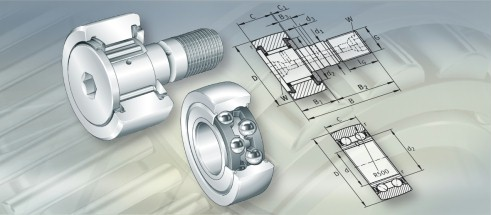
\includegraphics[width=\linewidth]{galet}
\end{center}


\begin{center}
 \includegraphics[width=.9\linewidth]{schema2}
\end{center}

\subparagraph{}
\textit{Quelle est la modification sur le paramétrage du système ?}
\ifprof%
\begin{corrige}

Un angle $\gamma$ correspondant à la rotation du galet sur lui même apparaît.

\end{corrige}
\else \fi

\subparagraph{}
\textit{Comment est-il possible de traduire l'hypothèse de \textbf{roulement} sans glissement ?}
\ifprof%
\begin{corrige}
La vitesse est nulle entre le galet et la croix de Malte est nulle au point $I$ :
$$ 
\vect{V(I,S_3/S_2)} = \vect{0}
$$
\end{corrige}\else\fi

\subparagraph{}
\textit{Calculer la vitesse de rotation du galet $\dot{\gamma}$ en commençant par exprimer $\vect{V(I,S_3/S_2)}$?}
\textit{Indice : décomposer $\vect{V(I,S_3/S_2)}$ en fonction des mouvements connus.}
\ifprof%
\begin{corrige}

Malgré l'introduction d'un nouveau composant, la position du point $I$ reste inchangée.

Il faut identifier le torseur $\{\mathcal{V}(S_3/S_2)\}$. 
Pour cela, la composition des vitesses donne :
$$
\{\mathcal{V}(S_3/S_2)\} = \{\mathcal{V}(S_3/S_1)\} + \{\mathcal{V}(S_1/S_2)\}  
$$


Au point $I$ on connaît déjà $\{\mathcal{V}(S_1/S_2)\}$.

Calculons $\{\mathcal{V}(S_3/S_1)\}$:

$$
\{\mathcal{V}(S_3/S_1)\}
= 
\left\{
\begin{array}{l}
\vect{\Omega(S_3/S_1)} = \dot{\gamma}\vect{z_0} \\
\vect{V(A,S_3/S_1)} = \vect{0}
\end{array}
\right\}_A =
\left\{
\begin{array}{l}
\vect{\Omega(S_3/S_1)} = \dot{\gamma}\vect{z_0} \\
\vect{V(I,S_3/S_1)} = \vect{IA} \wedge \dot{\gamma}\vect{z_0}
= -r\vect{y_2} \wedge \dot{\gamma}\vect{z_0} = -r \dot{\gamma}\vect{x_2}
\end{array}
\right\}_I
$$

On a donc :
$$
\vect{V(I,S_3/S_2)} = \vect{V(I,S_3/S_1)} + \vect{V(I,S_1/S_2)} 
$$
$$
\vect{V(I,S_3/S_2)} = -r \dot{\gamma}\vect{x_2} 
+\left(-r\dot{\beta}+ R\dot{\alpha}\cos(\alpha-\beta) + r\dot{\alpha}\right)\vect{x_2}
- \left(\lambda(t) \dot{\beta}+  R\dot{\alpha}\sin(\alpha-\beta)\right)\vect{y_2}
$$


$$
\vect{V(I,S_3/S_2)} =\left[ 
\begin{array}{l}
 -r \dot{\gamma}+\left(-r\dot{\beta}+ R\dot{\alpha}\cos(\alpha-\beta) + r\dot{\alpha}\right)\\
- \left(\lambda(t) \dot{\beta}+  R\dot{\alpha}\sin(\alpha-\beta)\right)\\
0\\
\end{array}
\right]_{\mathcal{R}_2}  
$$


%De même que précédemment, les solides étant indéformable, la projection de la vitesse sur $\vect{y_2}$ est nulle. 

D'après l'hypothèse de roulement sans glissement, on a :
$$ 
\vect{V(I,S_3/S_2)} = \vect{0} \Longrightarrow  \dot{\gamma}=-\dfrac{-r\dot{\beta}+ R\dot{\alpha}\cos(\alpha-\beta) + r\dot{\alpha}}{r}
$$

\end{corrige}
\else \fi

\subparagraph{}
\textit{Valider le choix du galet.}
\ifprof%
\begin{corrige}

$$
 \dot{\gamma}=-\dfrac{-r\dot{\beta}+ R\dot{\alpha}\cos(\alpha-\beta) + r\dot{\alpha}}{r}
$$
\end{corrige}\else\fi



\ifprof
\else
\end{multicols}
\fi


